%!TEX root = ../report.tex
\chapter{Architectural business information}
\label{ch:business}
The following section describes the different aspects of the business environment of the Smart Flood Monitor. First we will explain our vision and why there is place for us at the market. After this the product and its customers will be explained. This chapter is completed with a more detailed look at the business model and some models about the market and the financial prospect.

\section{Business opportunity}
There are many natural disasters happening each year all over the world. Each year these disasters take lives, waste a lot of properties and money and cause social disturbance. It is expected that natural disasters will cause \$300 billion in losses annually in the upcoming decade. Climate change causes the natural disasters to get worse every year. Also the number of natural disasters has increased significantly since 1970.\\
Looking at, for example, the Indian ocean's tsunami in 2004, it looks that the damage could have been significantly reduced if the necessary people were warned. A system that would reduce the damage of natural disaster, could result in billions. \\
A system that warns and guides the people before or during the floods can result in billions being saved and will save a lot of lives.

\section{Vision statement}
The Smart Flood Monitor will cause a revolutionary innovation on the environmental monitoring market. \CompanyName{} will offer a system which can detect floods early and correctly. This system helps us to enforce our vision, to limit the social and financial consequences of floods and avoid the loss of human lives. \\

\CompanyName{} will not be the only player on the environmental monitoring market as there are a lot of other competitors taking part on this area of expertise. This means \CompanyName{} will have to take their own strength and weaknesses into account. If we combine these qualities with an analysis of the opportunities and weaknesses on the market, we should be able to become a core part of the future environmental monitoring systems.\\

% Such an analysis is called a SWOT-analysis.
We try to map our position on the market by using SWOT-analysis. This analysis will map our strengths, weaknesses, opportunities, and threats as described as follows: 

% Strengths: Diverse team with several skills in IT and management. Experience with working with sensors.\\ 
% Weaknesses: No experience with creating such system. No knowledge of floods. The product is a complex system.\\
% Opportunities: Due to climate change, the market will grow and such a system becomes more urgent. Few competitors in the market. Smart sensors are a hot topic, new sensors will be developed.\\
% Threats: High production costs. Competitors will enter the market because of growing market. Climate change will force to improve the system over time.\\

\begin{description}
  \item[Strengths] \hfill \\
  Diverse team with several skills in IT and management. Experience with working with sensors.
  \item[Weaknesses] \hfill \\
  No experience with creating such system. Less knowledge about floods and environmental sciences. The product is a complex system.
  \item[Opportunities] \hfill \\
  Due to climate change, the market will grow and such a system becomes more urgent. Few competitors in the market. Smart sensors are a hot topic, new sensors will be developed.
  \item[Threats] \hfill \\
  High production costs. Competitors will enter the market because of growing market. Climate change will force to improve the system over time.
\end{description}

\newcommand{\SwotItems}[1]{
	\begin{itemize}
	%\begin{minipage}[t][8cm]{5cm}
		#1
	%\end{minipage}
	\end{itemize}
}
\begin{figure}
%Strengths
\newcommand{\Strengths}{
\SwotItems{
	\item Adjustable system that is future proof
	\item Having a low selling price. Lower then the competitors
	\item Diverse team with several skills in IT and management
	\item Having a good management team
	\item Frequent discussion with technical and business experts in the field.
	\item Experience with working with sensors
%	\item Main features don't focus on user-interaction.
%	\item Having a relatively big project team
%	\item Financial stability
}
}

\newcommand{\Weaknesses}{
\SwotItems{
	\item Decisions need to be made by the entire project team. There is a higher chance of a difference of opinion is members, holding back the project and leads to time wastes
	\item No experience with creating such system
	\item No knowledge of floods
	\item The product is a complex system
	\item Some main features rely on country-specific systems
}
}

\newcommand{\Opportunities}{
\SwotItems{
	\item Due to climate change, the market will grow and such a system becomes more urgent
	\item Few competitors in the market
	\item With a bigger program team, the pros and cons of the decisions are more clear
	\item Allowing the system to be flexible so it can also be used for other kinds of monitoring activities
%	\item Adding more ways the system can message the people in dangerous areas
%	\item Though the team doesn't have direct experience in this field, the team does have experience with specific parts of the system
	\item Smart sensors are a hot topic, new sensors will be developed. Making the system support and use the newest sensors allows it to obtain more, and a wider variety of valuable information
}
}

\newcommand{\Threats}{
\SwotItems{
	\item High production costs
	\item Competitors will enter the market because of growing market
	\item New competitors will enter the market
	\item Climate change will forces the system to be improved over time.
	\item Changes of the external systems that our system uses to properly communicate.
	\item The sizes of certain area{'}s to monitor can be too big to get a good and reliable view of them
}
}

\usetikzlibrary{matrix}

\colorlet{helpful}{lime!70}
\colorlet{harmful}{red!30}
\colorlet{internal}{yellow!20}
\colorlet{external}{cyan!30}
\colorlet{S}{helpful!50!internal}
\colorlet{W}{harmful!50!internal}
\colorlet{O}{helpful!50!external}
\colorlet{T}{harmful!50!external}

\newcommand{\texta}{Helpful\\ \tiny (to achieve the objective)\par}
\newcommand{\textb}{Harmful\\ \tiny (to achieve the objective)\par}
\newcommand{\textcn}{Internal origin\\ \tiny (product\slash company attributes)\par}
\newcommand{\textdn}{External origin\\ \tiny (environment\slash market attributes)\par}

\newcommand{\back}[1]{\fontsize{60}{70}\selectfont #1}

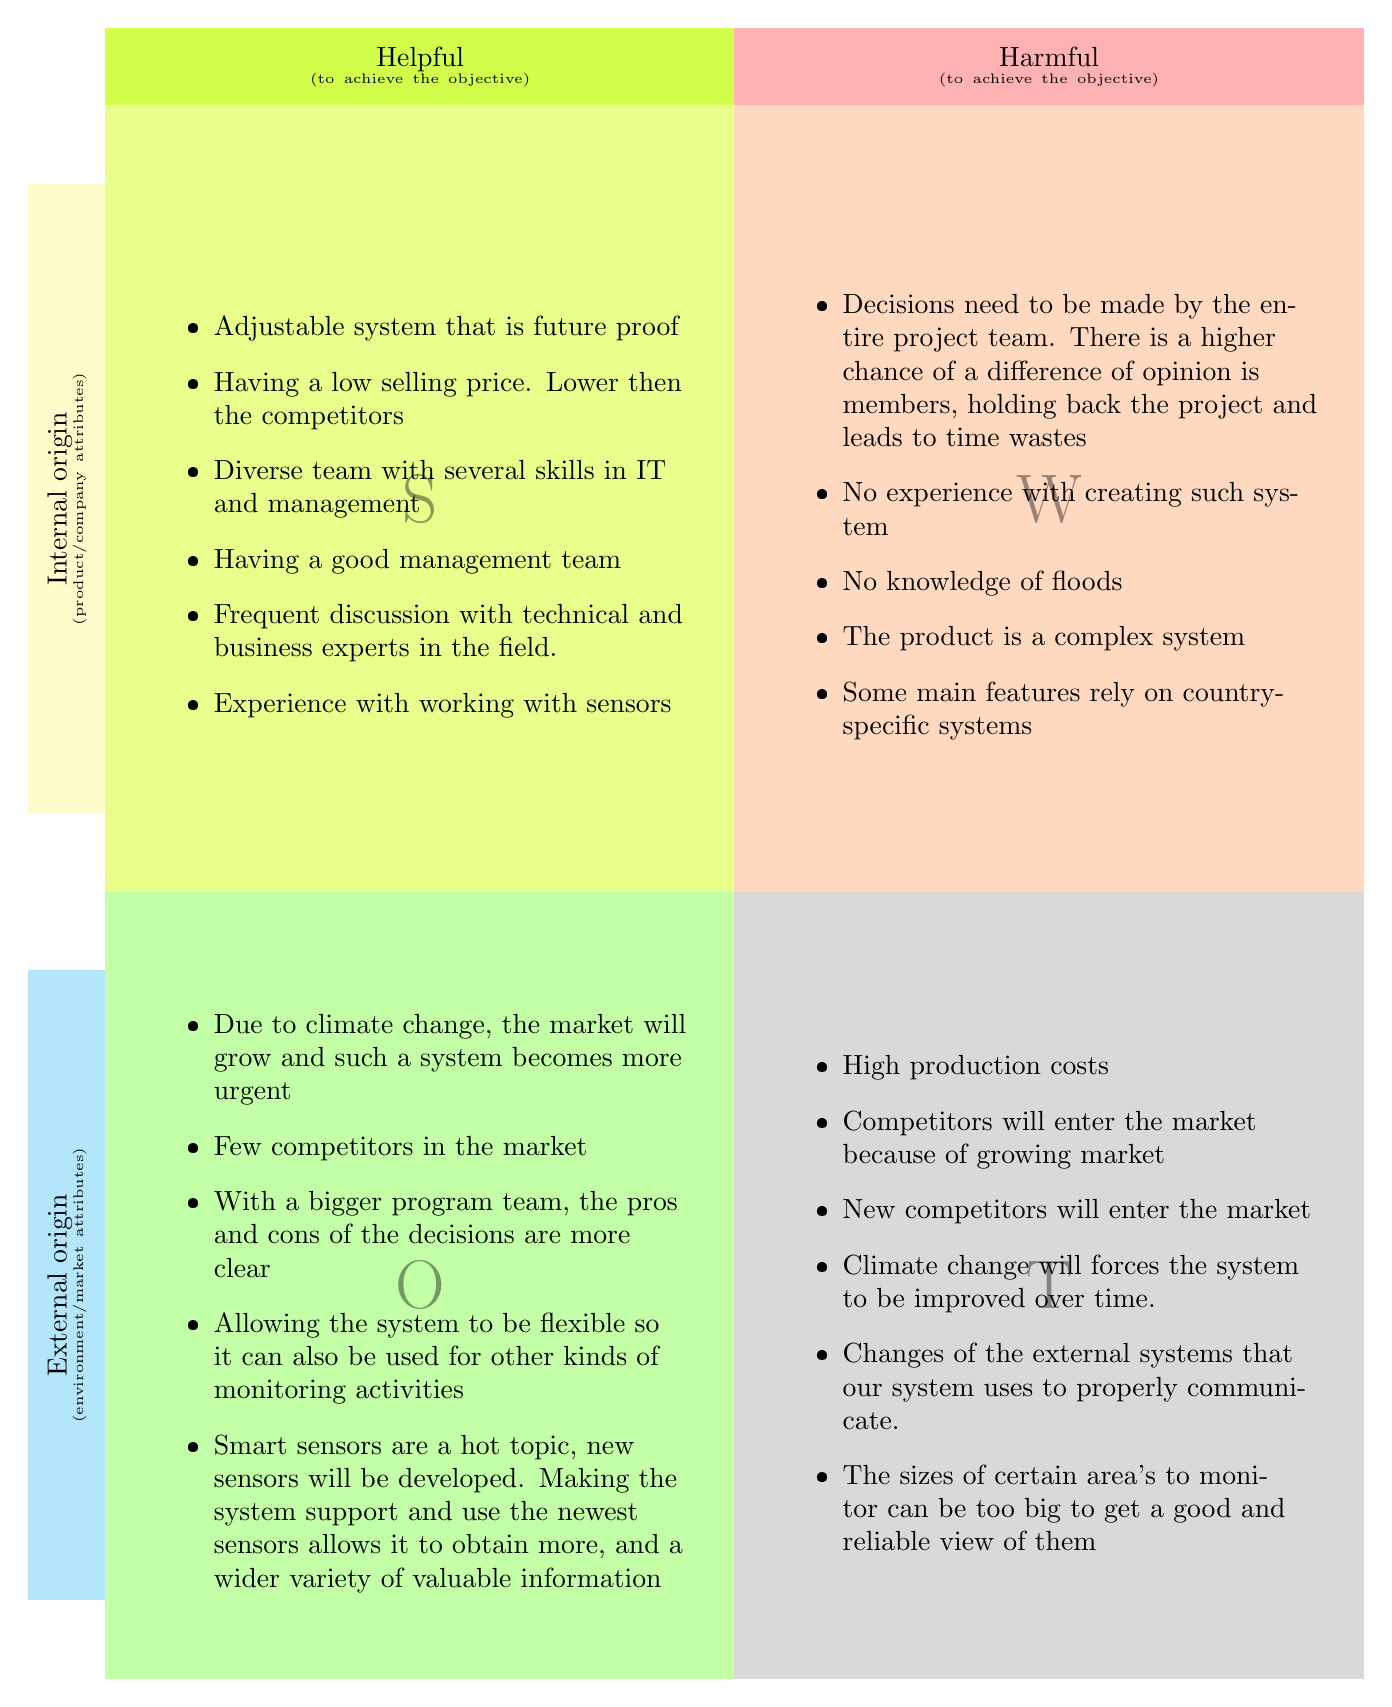
\begin{tikzpicture}[
    any/.style={minimum width=8cm,minimum height=10cm,%
                 text width=7cm,align=center,outer sep=0pt},
    header/.style={any,minimum height=1cm,fill=black!10},
    leftcol/.style={header,rotate=90},
    mycolor/.style={fill=#1, text=#1!60!black}
]

\matrix (SWOT) [matrix of nodes,nodes={any,anchor=center},%
                column sep=-\pgflinewidth,%
                row sep=-\pgflinewidth,%
                row 1/.style={nodes=header},%
                column 1/.style={nodes=leftcol},
                inner sep=0pt]
{
          &|[fill=helpful]| {\texta} & |[fill=harmful]| {\textb} \\
|[fill=internal]| {\textcn} & |[mycolor=S]| \back{S} & |[mycolor=W]| \back{W} \\
|[fill=external]| {\textdn} & |[mycolor=O]| \back{O} & |[mycolor=T]| \back{T} \\
};

%\node[below right, any] at (SWOT-2-2.north west) {\Strengths};
\node[any, anchor=center] at (SWOT-2-2) {\Strengths};
\node[any, anchor=center] at (SWOT-2-3) {\Weaknesses};
\node[any, anchor=center] at (SWOT-3-2) {\Opportunities};
\node[any, anchor=center] at (SWOT-3-3) {\Threats};
\end{tikzpicture}
\caption{SWOT-analysis diagram.}
\label{fig:swot}
\end{figure}

Our unique selling point is to provide a system with low selling price and high profit from the service contracts and upgrades.

\section{Business rationale}
\CompanyName{} will develop a new flood warning system in order to minimize the damage caused by a flood. In the Netherlands protection against floods is an important issue, because the position of the Netherlands itself is actually below sea level. Global warming will increase the urgency of this issue. The people within the Netherlands must be well protected against floods. The flood warning system will detect floods, warn people and governmental institutions located in the disaster area and provide guidance where to go to. \todo{truncated}
\\
\CompanyName{} is new within the flood warning system market. By using sensors and automated systems, a reliable and adequate product that uses of the newest technologies will be launched. \CompanyName{} will use hardware which is already on the market and is tested. Buying third party hardware will also speedup the development of the system and lower the costs.\\

The product price will be low in order to get a market share and prove the product in a real-time environment. By providing maintenance and updates in the future \CompanyName{} will earn money to improve the product further and sell it to other potential customers. This in combination with the increasing need of a reliable warning system for imminent floods will result in a viable business.\\


The unique selling points of our system are: 
\begin{itemize}
	\item To provide a system with low selling price and high profit from the service contracts and upgrades.
	\item Warn the people in and around the area as soon as possible if the system is very certain that a flood is or will happen.
	\item Inform people about the details of the flood so the right preparations are made. 
	\item Inform people how to save themselves, others or goods.
\end{itemize}

This way, people will know when an area gets flooded, or when it is about to happen. People who requested it, will get informed on how to prepare for the flood and what to do during the flood.\\
These features are things that are be unique for our system and that make it successful. The main goal of this project, however, is to safe lives, reduce costs and reduce social consequences. These main goals will be met when:
\begin{enumerate}
	\item 80\% of the people in a dangerous area regarding a flood, receive a warning message. This message must contain enough information for receivers to know whether they are save or not and if not, how they can get to a save location.
	\item 80\% of the people who receive a warning successfully get to a safe environment in time.
	\item 80\% of the people receiving information before or during a flood, find these messages helpful and reported that it guided them successfully in order to save extra lives and/or goods.
\end{enumerate}

When the first version of \ProjectName{} is released and is used to start monitoring actual floods, its success will be measured according these statistics. Getting a warning message to the people who need to be warned is the most important thing to do. Using this warning message, people can move to a saver location.

\subsection{Scope of Initial and subsequent releases}
%\todo{If you want to make this distinction you should mention the functionality of the first version too. Use some charts to show the progress during time from business and technical perspective.}

The initial release will only focus on floods as a natural disaster. It will send warnings to the necessary people, but will not yet interact much with the user. The system, however, doesn't stop there, and will get increasingly more capabilities. The extra capabilities of system include:
	\begin{itemize}
		\item Support for more kinds natural disasters
		\item More individual guidance
		\item Interaction with the system, users can give input
		\item Adding more sensor support
		\item Using multiple communication networks to send information
	\end{itemize}

The first thing \CompanyName{} will focus on after the first release, is to let users interact with the system more. This will allow the system to have better knowledge of the area. However, mistakes can easily be made by a user and so this data needs to be verified in order to get valuable information. That is why adding this feature goes beyond the scope of this project.\\
Adding sensor support is a continuous process. The sensors that are available are steadily increasing and their technology becomes more advanced. \CompanyName{} will monitor the sensor technologies and improvements to check if these can improve the system. \\
Depending on where the system resides, it will need to interact with various kinds of networks en media. Initially the flood warning system will focus on communicating with resources in the Netherlands. However, if a future release implements additional support for monitoring tornadoes or volcanoes, the system will most likely not be in the Netherlands.

\begin{figure}[h!]
  \centering
    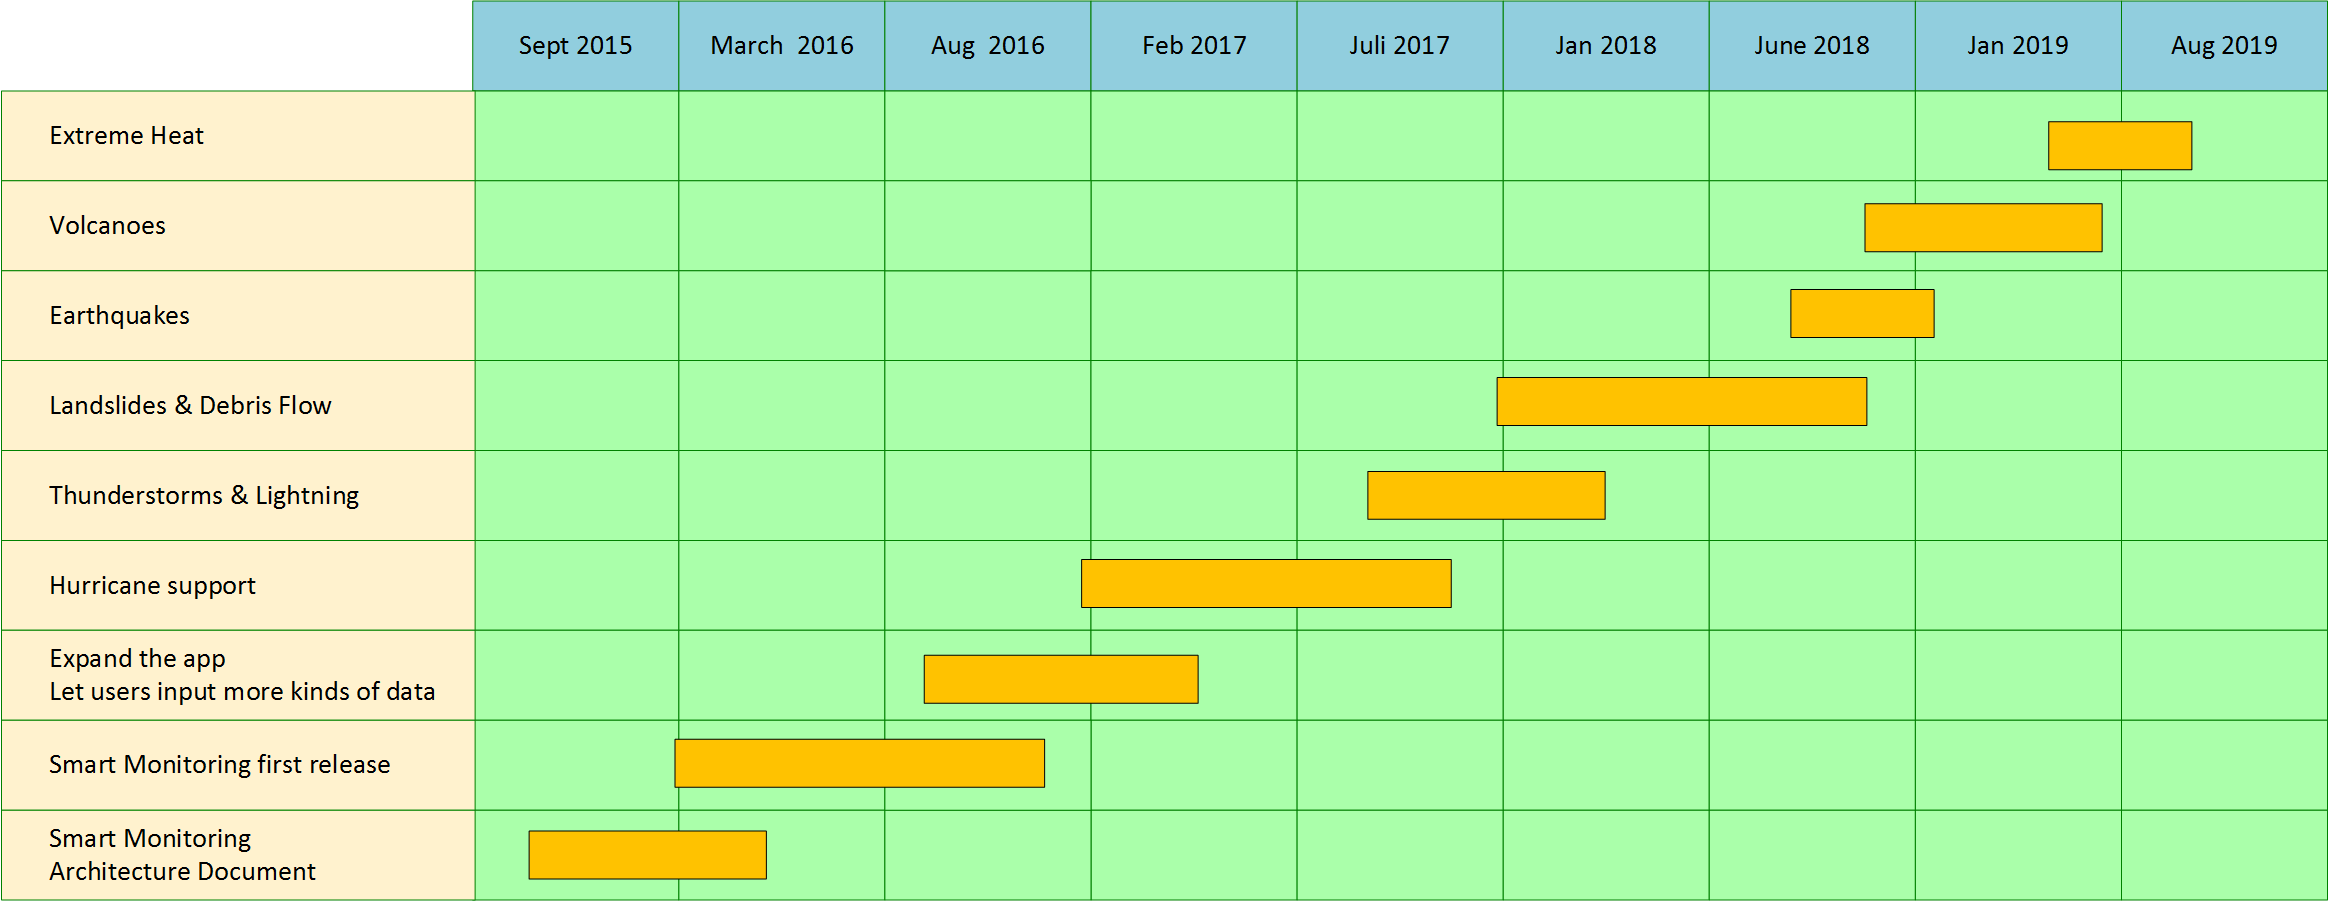
\includegraphics[width=0.95\textwidth]{{{2-business/images/release}.png}}
   \caption{Future releases.}
   \label{fig:future-releases}
\end{figure}


%\section{Business rationale}
\section{Product and service description}
\CompanyName{} offers a flood warning system. When a imminent flood is monitored by the sensors of the system a warning should be sent to governmental organizations and people within the danger area. Also guidance should be provided when a flood is happening to assist rescuers and guide inhabitants to safe areas.\\

Basically the system will consist of four subsystems: monitor the state of dykes and water levels, monitor if a imminent flood is occurring, warn governmental organizations and inhabitants in the danger area, and provide guidance to search and rescue organizations and inhabitants.\\

The first subsystem, monitor the state of dykes and water levels, will consist of various sensors that are placed near and in dykes and water ways. The state of the dikes must be monitored continuously, i.e. pressure of the dyke. Also, sensors must be installed to monitored continuously the water level. The data of all the sensors will be sent to a server, in a safe location, to store all the data.\\

The second subsystem, monitor if a imminent flood is occurring, will analyze all the data from the sensors and data from weather forecasting service. Based on this data an algorithm will monitor continuously if there are dangerous situations.\\

The third subsystem, warn governmental organizations and inhabitants in the danger area, will send warning messages when the algorithm identified a dangerous situations. The safety region ---in Dutch Veiligheidsregio--- will receive a warning message that an area is in danger. Information like place, sort danger and amount of danger will be send. The safety region will be responsible to take action based on this information. Inhabitants can receive warnings via sirens, mobile phone, radio, television, and by UAV.\todo{truncated}

The last subsystem, provide guidance to search and rescue organizations and inhabitants, will help people that are in the danger area how to flee and rescue in a save way. Rescue organizations will receive information where are probably the most casualties and how to get safe to those locations.\\


The service will consist of maintenance for the product and upgrades.

\section{Target audience}
The Dutch Ministry of Infrastructure and the Environment is the target customer. They have the responsibility in the government to identify unsafe situations caused by floods. When this ministry wants a new warning system they need to start a procurement. This gives the opportunity for various companies to bid on the procurement. At first the Dutch Ministry is our target audience, later on the product can be sold to other countries.

%\section{Business model}
%\ Insert a business model diagram
%\section{Roadmaps}
%\ How to enter the market

\section{Road maps}
The Dutch Ministry of Infrastructure and the Environment will end the procurement of a flood warning system on 31-12-2015. The bid must consists of the design of the system and a financial analysis must be made. The engineering part of the system will be finished on 31-12-2016. An operating system is then up and running.

Directly after finishing the initial product, new features will be developed and can be sold.

After this first step there will tried to market the system to other countries in the world. 
% Guntur: Two target audience sections?
% \section{Target audience}
% The product will be sold to governmental institutions. 

%\section{Business model}
%\ Insert a business model diagram
%\section{Roadmaps}
%\ How to enter the market
\section{Financial model}
The financial model will be a low product price. This in order to price the product low in the market. A service description for maintenance will be offered. Also updates will be sold to the customer

\subsection{Software Architecture costs}
The software architecture team consists of seven members. The project will last 10 weeks. All team members will spend 15 hours a week on the project. This totals 1050 working hours. Each working hour costs \euro{}150,-. Total spend on the software architecture is \euro{}157.500
\subsection{Development costs}

\subsection{Hardware costs}

\subsection{Total costs}

% Guntur: Doubled financial model sections?
% \section{Financial model}
% The financial model will be a low product price. This in order to price the product low in the market. A service description for maintenance will be offered. Also updates will be sold to the customer

\section{Competitors}
Siemens designed a flood-warning system via SMS in Belgium.
%http://datanews.knack.be/ict/nieuws/sms-waarschuwt-voor-overstromingen-br/article-normal-317597.html
%http://www.urbanflood.eu/Pages/Newsletter6.aspx

